% P34 Figure: computation / transputation boundary
\begin{figure}[htbp]
\centering
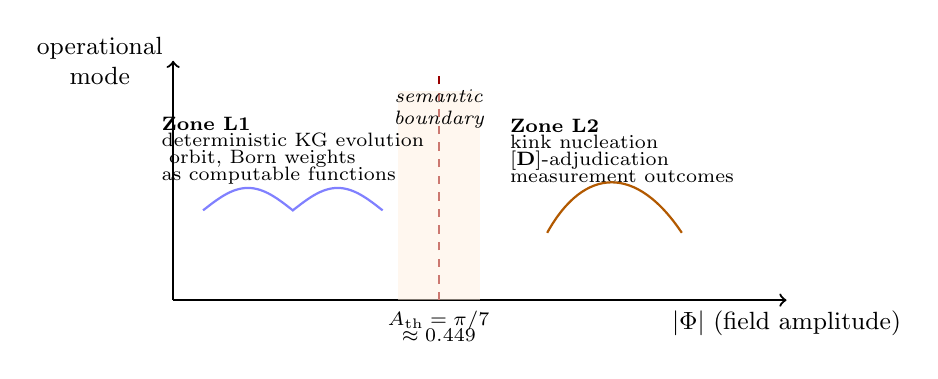
\begin{tikzpicture}[scale=0.95, every node/.style={font=\small}]
  \draw[->,thick] (0,0) -- (8.2,0) node[below] {$|\Phi|$ (field amplitude)};
  \draw[->,thick] (0,0) -- (0,3.2) node[left,align=center] {operational\\mode};
  % Threshold
  \draw[dashed,thick,red!60!black] (3.55,0) -- (3.55,3.0);
  \node[font=\scriptsize,align=center] at (3.55,-0.35)
    {$A_{\mathrm{th}}=\pi/7$\\[-2pt]$\approx 0.449$};
  % Gradient band
  \fill[orange!12,opacity=0.5] (3.0,0) rectangle (4.1,2.8);
  \node[font=\scriptsize\itshape,align=center] at (3.55,2.55) {semantic\\boundary};
  % Zone L1
  \node[align=left,font=\scriptsize] at (1.6,2.0)
    {\textbf{Zone L1}\\[-2pt]deterministic KG evolution\\[-2pt]$\fmdl$ orbit, Born weights\\[-2pt]as computable functions};
  \draw[thick,blue!50] (0.4,1.2) sin (1.0,1.5) cos (1.6,1.2)
    sin (2.2,1.5) cos (2.8,1.2);
  % Zone L2
  \node[align=left,font=\scriptsize] at (6.0,2.0)
    {\textbf{Zone L2}\\[-2pt]kink nucleation\\[-2pt]$[\mathbf{D}]$-adjudication\\[-2pt]measurement outcomes};
  \draw[thick,orange!70!black] (5.0,0.9) .. controls (5.5,1.8) and (6.2,1.8) .. (6.8,0.9);
\end{tikzpicture}
\caption{On the $\Phi_{\mathrm{MDL}}$ field, bounded sub-threshold evolution is
  Turing-decidable (Zone~L1); above-threshold kink formation and individual
  measurement outcomes require transputation (Zone~L2). The boundary is set by
  field amplitude, not by syntax alone.}
\label{fig:comp_transputation_boundary}
\end{figure}
